\documentclass[11pt,a4paper]{article}
\usepackage{ifpdf}
\usepackage[utf8]{inputenc}
\usepackage[francais]{babel}
\usepackage[T1]{fontenc}
\usepackage[nottoc, notlof, notlot]{tocbibind}
\usepackage[unicode=true,pdftex,colorlinks=true,linkcolor=black,urlcolor=black,citecolor=black]{hyperref}
\usepackage{natbib}
\usepackage{graphicx}

\parindent 0.8cm
%\setlength{\parskip}{0.5em plus 0.2em minus 0.2em}

\title{Projet HADL}
\author{Anthony \textsc{Caillaud} Manoël \textsc{Fortun}}
\date{\today}
\ifpdf
\pdfinfo {
/Author (Anthony Caillaud Manoël Fortun)
/Title (Projet HADL)
/Subject (Projet HADL)
/Keywords ()
/CreationDate (D:20100329212218)
}
\fi


\begin{document}

\maketitle


\clearpage
\tableofcontents
\clearpage
\section{Introduction}

Dans le cadre de notre module Composants dans lequel nous avons pu étudier les
modèles à composants et leurs fonctionnements, nous avons du modéliser et écrire
notre propre langage d'architecture logicielle à composants. Ce projet ne
consistait pas seulement en la définition d'un langage d'architecture à
composants, mais aussi en l'implémentation en langage objet d'un moteur
d'architecture à composants. Ce rapport présente donc le travail que nous avons
pu effectuer sur cet HADL(home architecture definition langage). Dans un
premier temps, le travail de modélisation des concepts composants
(meta-modélisation) ainsi que l'implémentation du modèle vous sera présenté.
Ensuite, l'application du modèle à composants (modélisation) vous sera
expliquée à travers l'exemple du système Client/Serveur. Enfin, nous
détaillerons le meta-meta-modèle que nous avons pu définir pour notre HADL.


\section{Description du méta-modèle HADL}
\subsection{Définitions}
L'architecture logicielle à base de composants est consitutés de trois
principaux éléments : des composants, des configurations et des connecteurs.\\

\subsubsection{Eléments principaux}

% - Def Composant
 Un composant est une unité de composition qui spécifie une ou plusieurs
 fonctionnalités. Celui-ci peut être déployé indépendemment, il s'agit de la
 brique élémentaire.\\

%- Def Configuration
Une configuration est un ensemble de composants et de connecteurs, il définit la
façon dont ils sont reliés entre eux. Cette unité de l'architecture logicielle
à base de composants est nécessaire aux bonnes liaisons entre composants. Elle
permet de savoir si ces liaisons relatives aux connecteurs permettent une
communication correcte. C'est la configuration qui gère tous les composants et
tous les connecteurs qui la composent.\\

%- Def Connecteur
Un connecteur explicite est une unité effectuant une liaison entre des
composants ou des configurations. Les connections proprement dites s'effectuent
grâce à des Rôles (Rôles From et Rôles To) et une ''Glue'' qui représente la
fonction modifiant les informations transférées. Il peut être comparé à un
adaptateur entre deux composants.\\

\subsubsection{Eléments secondaires}

%-Def Interface 
L'interface d'un composant, connecteur ou configuration est l'ensemble des
éléments fournis pour l'intéraction avec le composant, connecteur ou
configuration. Il s'agit plus d'un concept que d'un élément concret. Une
interface est généralement constituée de ports et de services.\\

%- Def Port
Un port est un point d'entrée ou de sortie d'un composant ou configuration, il
pourrait s'apparenter à un attribut d'une classe si on fait le rapprochement
entre le modèle composant et le modèle objet.\\

%- Def  Service
Un service est une opération disponible auprès d'un composant, il y a des
services fournis par un composant et des services requis pour son fonctionnement.
Un service peut être assimilé à une méthode toujours dans le parallèle
composant/objet. Un service peut être relié à des ports ce qui signifie que
certains ports seraient les entrées du service et d'autres ports seraient la ou
les sorties du service.\\

%-Def Propriétés
Les propriétés sont des éléments appartenant aux configurations ou composants,
les propriétés peuvent définir une particulatité du comportement ou un élément
dont on peut se servir, comme un attribut de classe.\\

%-Def Contraintes
Les contraintes sont des éléments importants, puisque elles définissent ce dont
ont besoin les composants ou configurations pour fonctionner,  par exemple la
présence d'une librairie particulière.\\

%-Def Roles
Ce concept est propre aux connecteurs, il y a les roles from et role to qui
constituent l'interface des connecteurs, leurs entrées et leurs sorties.\\

%-Def Lien
Les liens sont des éléments qui permettent de relier des composant entre eux, ou
une configuration à un composant. On distinguera deux types de liens:
\begin{itemize}
  \item Les attachements qui sont des liens entre composants, lien qui inclut un
connecteur,
  \item Les bindings qui relient les ports de configuration aux port de
  composant, lien qui n'inclut pas de connecteur.
\end{itemize}
 
\subsection{Analyse}

Pour l'implémentation de notre HADL, nous avons du modéliser le meta modèle (niveau M2) à l'aide de l'uml puisque l'objectif était d'avoir une implémentation objet du HADL. Pour ce faire nous avons commencer à mettre en rapport les concepts liés.

Comme le fait que composant, connecteur ou configuration seraient des classes puisque représentant des éléments majeur de l'architecture à composant. Et donc pour l'implémentation d'une véritable architecture les composants hériterais de ce meta modèle.

Les configurations sont un assemblage de composant et de connecteur, une composition de ces éléments dans la configuration. De la même manière que ces éléments sont des classes, nous avons considéré que les liens étaient aussi important pour eux aussi être des classes. Par conséquent la classe configuration est aussi composé de lien.

La classe configuration est au centre de toute architecture puisque c'est elle qui contient la façon dont les composants interragissent entre eux. La classe configuration doit intercepter tout ce qui entre et sort des composants pour organiser le routage entre composant des différents messages, c'est une sorte de chef d'orchestre. Pour que ce soit le cas tout les éléments (connecteur, configuration et composant) seront des entités observable, et les configurations seront observateur de manière à observer tous les éléments qu'une configuration contient.

Configuration et composant sont des éléments très similaires ils disposent d'éléments commun comme des ports, propriétés et contraintes. Les configurations sont composé de composant et partagent des éléments communs, nous avons reconnu le pattern composite, comme nous le détaillerons au travers des diagrammes.

Le sujet suggèrait que l'on puisse remplacer des composants d'une configuration à tout moment, pour celà il faut que chaque appel d'un port ou service soit capturé par la configuration et que si l'action ne peut être éxécuté l'action soit entreposé et rééxécuté lorsque le composant ou connecteur manquant est de nouveau disponible.

Une partie du travail était aussi de gérer un véritable langage, un peu à la façon d'acme, le plus simple à été de créer une dtd et un parseur xml qui permet d'écrire des configurations en xml. 

Dans notre application les ports sont identifiés par des identificateurs numériques, et servent pour l'appel des services des composants. Les services sont en fait des méthodes d'instance, qui sont reliés aux ports.

\subsection{Diagrammes}

Le diagramme \ref{Premier meta-modèle} est notre première version du meta modèle du HADL. On peut voir les différents concept et la façon dont ils s'articulent autour des configurations et composants. Dans ce diagramme les concepts sont représenté, mais sans le parrallèle avec le model objet, comme le fait que les ports sont des attributs des objets.

\begin{figure}[h]
  		\centering
  		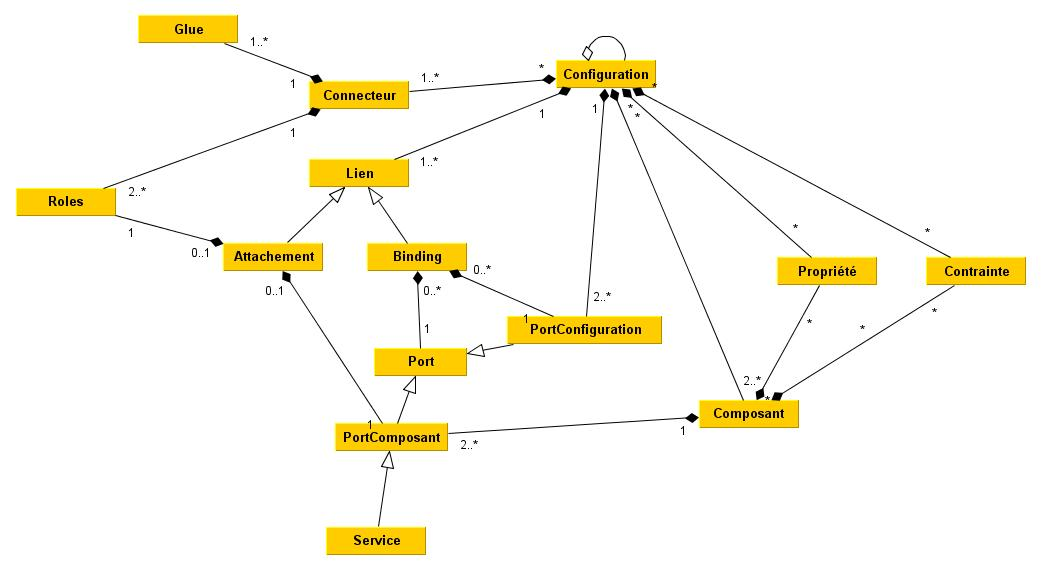
\includegraphics[height=14cm,width=15cm]{M2.jpg}
  		\caption{Premier meta-modèle}
  		\label{Premier meta-modèle}
\end{figure}


Le diagramme \ref{Meta modèle-objet} représente le meta modèle en objet. On peut y voir le pattern composite appliqué pour les configurations et composants, avec un niveau d'abstraction supérieur pour ces éléments reprenant l'ensemble des méthodes et attributs commune.

\begin{figure}[h]
  		\centering
  		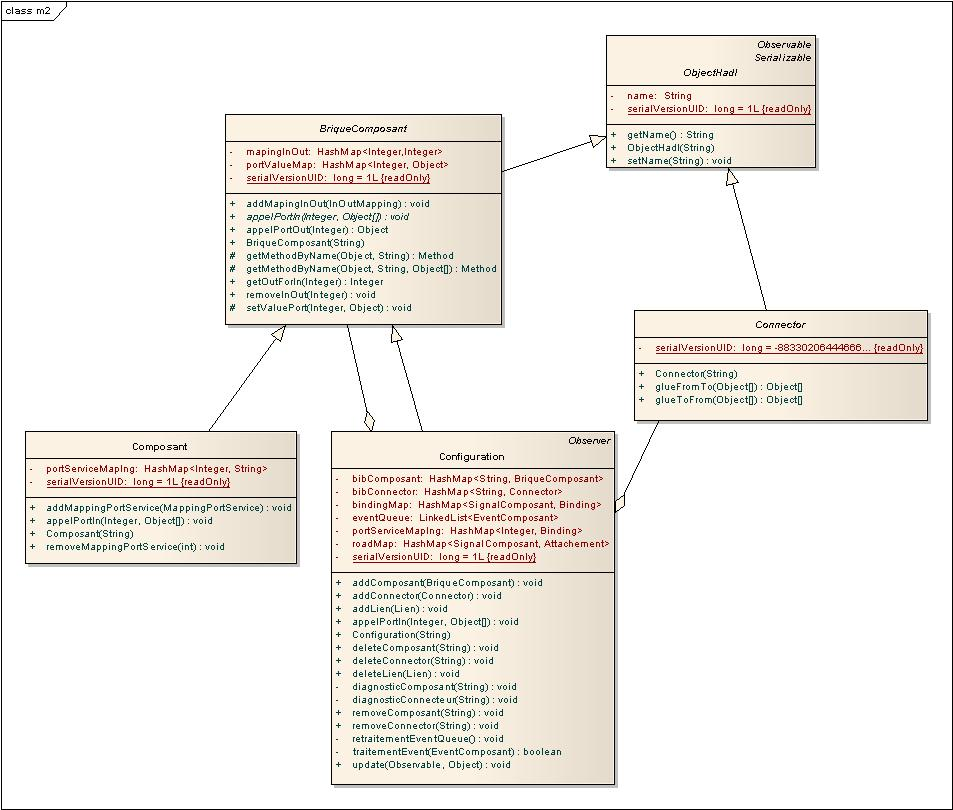
\includegraphics[height=14cm,width=15cm]{m2impl.jpg}
  		\caption{Meta modèle-objet}
  		\label{Meta modèle-objet}
\end{figure}


Ce diagramme \ref{Meta modèle-objet} montre aussi la représentation des ports qui sont en fait des valeurs enregistré dans une map pour les ports de sortie et pour les ports d'entrée un mapping permettant d'appeler les services des composants ou transferer les appels des ports configuration vers composants. La méthode appelPortIn sert pour l'invocation d'un service correspondant(mappé) sur un port numéroté avec des paramètres. Cette même méthode préviens l'observateur de son éxécution, en donnant le nom de l'élément et le nom de la méthode éxécuté, l'observateur ensuite regarde si cette notification corresponds à un binding ou un attachement. 

On peut aussi voir que tous les éléments de l'architecture hérite d'une abastraction objet hadl, qui contient l'attribut commun à tous les autres, un nom, qui permet de les identifier et de faire fonctionner l'architecture. 

\begin{figure}[h]
  		\centering
  		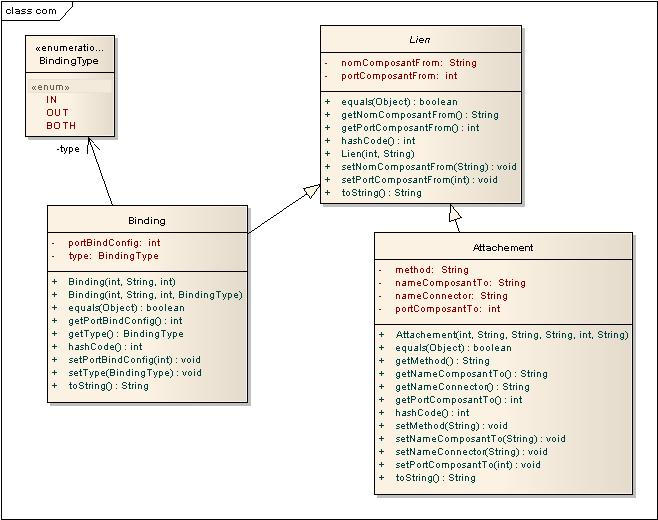
\includegraphics[height=14cm,width=15cm]{comimpl.jpg}
  		\caption{Représentation des liens}
  		\label{Représentation des liens}
\end{figure}

Sur le diagramme \ref{Représentation des liens} on peut voir la représentation des éléments de type lien, on peut y voir l'importance des noms qui permettent de définir les échanges entre composant avec connecteur. Ces noms servent à la configuration pour l'orchestration de son fonctionnement, et sa reconfiguration éventuel en changeant un composant ou connecteur.

Enfin le diagramme \ref{Représentation des Ports et Services} on peut y voir les classes permettants de configurer les composants, le mapping entre port et service d'un composant, et le mapping entrée sortie pour les ports, l'appel d'un service via un port écrira le résultat sur la sortie correspondante.


\begin{figure}[h]
  		\centering
  		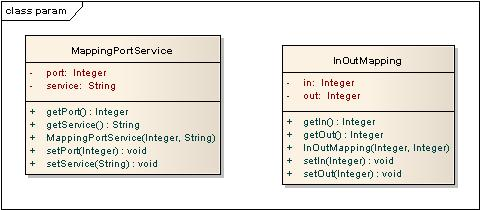
\includegraphics[height=14cm,width=15cm]{param.jpg}
  		\caption{Représentation des Ports et Services}
  		\label{Représentation des Ports et Services}
\end{figure}


\clearpage
\section{Description du système Client/Serveur}
\subsection{Définitions}
Le système Client/Serveur est une bonne représentation au niveau M1 d'une
architecture logicielle à composants. En effet, chacune des partie constituant
ce système peut être vu comme un composant faisant partie d'une configuration
représentant celui-ci. Ces trois composants principaux sont le client, le
serveur et le connecteur RPC qui permet la communication entre les deux
premières entités.\\

Le client est donc un simple composant de la configuration ''Client/Serveur''
permettant l'envoi et la réception de messages. Le serveur, quant à lui, est
une configuration comprenant plusieurs autres composants permettant le
traitement du message reçu.


\subsection{Analyse}
Au niveau M1, chacun des composants offre des services. Tout d'abord, le
client permet donc d'envoyer et de recevoir des messages. Ces deux services
sont liés à deux ports différents.\\


Les trois composants de la configuration ''Serveur'' sont ConnectionManager,
SecurityDB et Database.
 
ConnectionManager est le composant qui va recevoir en premier le message envoyé
par le client. En effet, via un lien Binding, c'est ce composant qui communique
avec la configuration ''Serveur''. Dans notre implémentation, il propose deux
services indiquant l'entrée et la sortie du message dans le composant.

Le composant SecurityDB est celui qui effectue des vérifications liées à
la sécurité et aux autorisations concernant le message provenant du client.
Nous avons choisi de ne pas implémenter de sécurité pour les messages que nous
voulions faire circuler. Le composant affiche uniquement un message dans le
terminal signalant le passage du message dans celui-ci. 

Enfin, le composant Database représente la base de données interrogée. Pour
cela, nous avons mis en place une HashMap avec quelques entrées. Un service de
ce composant est de renvoyer la valeur contenu dans la Map correspondant à la
clé reçue.\\

Tous ces composants, qui forment le Serveur, sont reliés entre eux à l'aide de
connecteurs. Ces connecteurs sont donc au nombre de trois : ClearenceRequest,
SecurityQuery et SQLQuery. La Glue de chacun de ses connecteurs ne fait que
transmettre le message, aucune autre action n'est effectuée sur le message.

ClearenceRequest fait le lien entre les composants ConnectionManager et
SecurityDB. Quant à lui, le connecteur SecurityQuery relie SecurityDB et
Database. Enfin, SQLQuery permet aux composants ConnectionManager et Database
de communiquer.\\

RPC est lui aussi, comme les autres connecteurs décrits précédemment, un
connecteur dont la Glue n'effectue uniquement la transmission du message entre
le composant Client et la configuration Serveur.

\clearpage
\subsection{Diagrammes}

\begin{figure}[h]
  		\centering
  		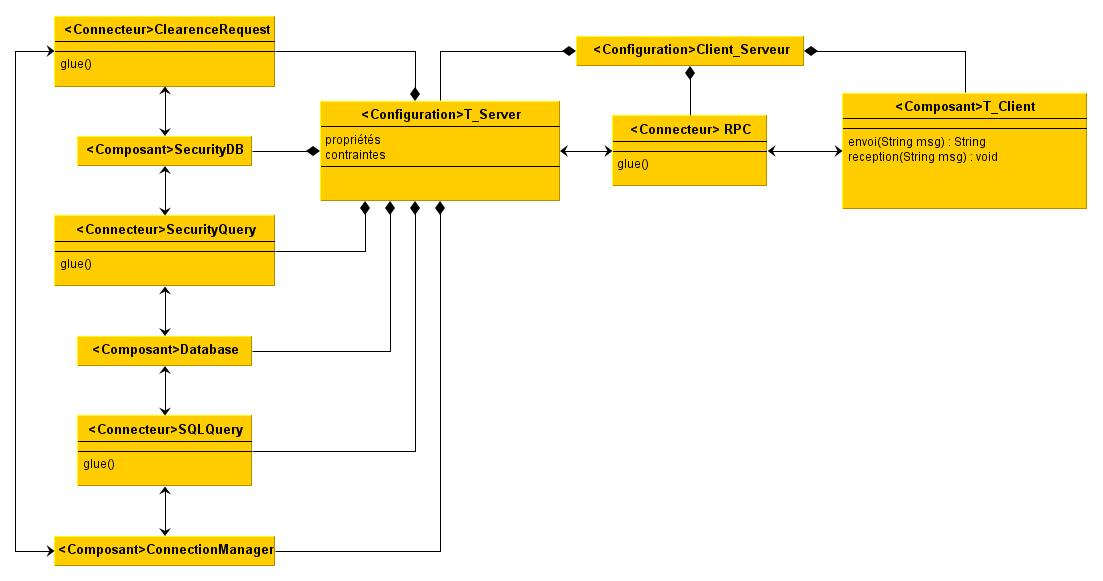
\includegraphics[height=14cm,width=15cm,angle=90]{M1.jpg}
  		\caption{Diagramme du système Client/Serveur}
  		\label{Diagramme du système Client/Serveur}
\end{figure}

\clearpage


\section{Description du méta-méta-modèle HADL}
\subsection{Définitions}
%- Def Meta-Entité
Une méta-entité correspond à une entité comme un composant ou une
configuration à un niveau d'abstraction plus grand qu'au niveau méta-modèle.\\

%- Def Meta-Relation
Une méta-relation correspond, de manière similaire à la méta-entité, à une
relation comme un lien d'attachement, un binding ou encore un lien de
composition à un niveau d'abstraction plus grand qu'au niveau méta-modèle.\\

%-Def 
Le meta meta modèle permet de se définir lui même de la même façon que pour le meta meta modèle objet, celà est rendu possible grace aux deux méta relations l'héritage et la composition qui sont les deux concepts essentiel des architectures à composant.

\subsection{Analyse}
Pour réaliser ce méta-méta-modèle, nous nous sommes aidé de l'exemple du
méta-méta-modèle des Langages Orientés Objets étudié en cours.

Deux méta-entités ont été définis dans notre diagramme : Composant et
Configuration et deux méta-relation : composant-de et meta-lien.

La méta-relation composant-de représente la composition effective entre la
notion de Composant et celle de Configuration. La relation méta-lien peut-être
vu comme le lien qu'effectue un connecteur entre deux composants, deux
configurations ou encore entre un composant et une configuration.

Nous avons choisi pour ce méta-méta-modèle de ne pas inclure tous ce qui concerne
les ports, services et d'autres notions afin de ne pas surcharger le diagramme.
Ces notions omises au niveau M2 telles que les ports et services sont des
méta-entités et les liens tels que les attachements et les bindings sont des
méta-relations.
\subsection{Diagrammes}

\begin{figure}[h]
  		\centering
  		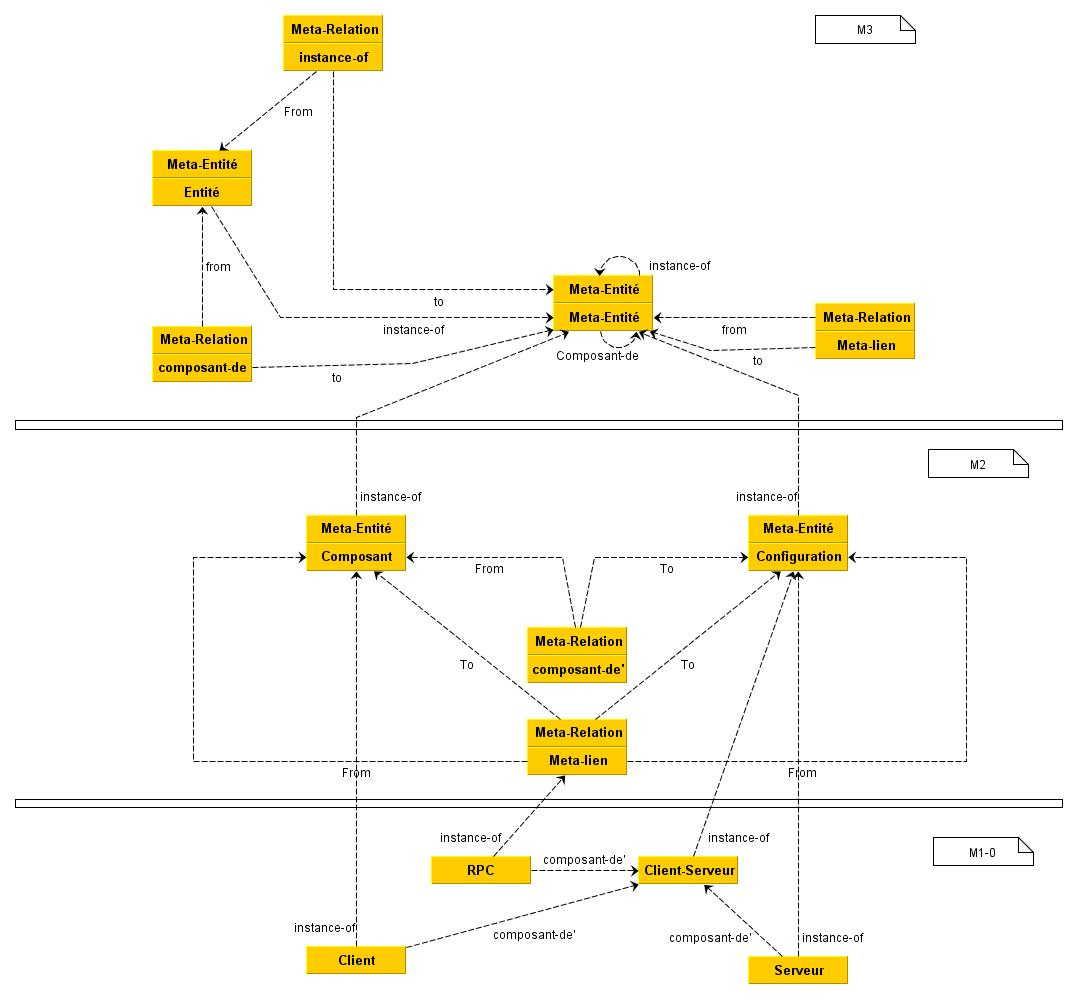
\includegraphics[height=14cm,width=15cm]{meta-meta-modele.jpg}
  		\caption{Diagramme du méta-méta-modèle HADL}
  		\label{Diagramme du méta-méta-modèle HADL}
\end{figure}


\section{Conclusion}

En conclusion, le travail effectué sur cet HADL nous a permis de bien observer
et de bien comprendre les différents niveaux d'une architecture logicielle à
composants. Ceci nous a permis de voir les différents niveaux d'abstraction
d'une architecture logicielle et ce qui les relient. De plus, l'implémentation
de la méta-modélisation jusqu'à l'instanciation nous a permis de voir
concrètement ces niveaux.


\end{document}
